\subsection{Neural Networks}

    \begin{figure}[H]
        \centering
        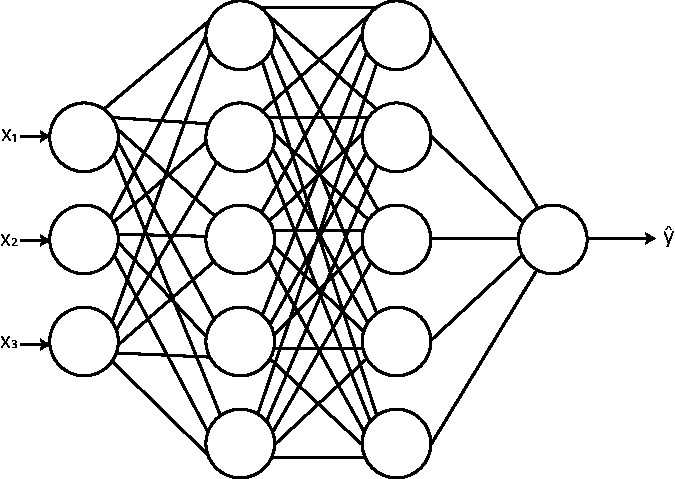
\includegraphics[width=\linewidth]{mlp.pdf}
        \caption{A very simple neural network; A fully connected multi-layer perceptron with 2 hidden layers and one output layer. The vector $\boldsymbol{x}$ is the input ($\boldsymbol{x} \in \rm I\!R^{3}$) and $\hat{y}$ is the output}
        \label{fig:simple_neural_network}
    \end{figure}
        
    Neural networks solve problems by learning optimal parameters to map a set input samples onto given output labels. They consist of layers which in turn consist of individual cells called neurons. Each neuron linearly transforms its output and then passes the output through a non-linear function to produce its activation which is its output. A simple neural network is shown in \autoref{fig:simple_neural_network}. The neural network shown is known as a fully connected multi-layer perceptron (MLP). Layers in such a neural network can be expressed using simple matrix multiplication:
    
    \begin{equation}
        \begin{split}
            \boldsymbol{z}_k &= \boldsymbol{W}_k \boldsymbol{a}_{k-1} + \boldsymbol{b}_k \\
            \boldsymbol{a}_k &= f\left(\boldsymbol{z}_k\right)
        \end{split}
    \end{equation}
    
    where $\boldsymbol{W}_k$ and $\boldsymbol{b}_k$ are the weight matrix and the bias vector for layer $k$ respectively. $\boldsymbol{a}_{k-1}$ is the activation of the previous player with $\boldsymbol{a}_{0}$ representing the input vector to the MLP. $\boldsymbol{z}_k$ is the result of the linear matrix multiplication which is then passed through a non-linear activation function $f\left(\boldsymbol{z}\right)$ which produces the activation of the layer $\boldsymbol{a}_{k}$.
    \\
    
    Some examples of non-linear activation functions are given in \autoref{eqn:activation_functions}:
    
    \begin{equation}
    	\label{eqn:activation_functions}
    	\begin{split}
    		f_{ReLU}(\boldsymbol{z})_i &= \max(0,z_i)\\
    		f_{tanh}(\boldsymbol{z})_i &= \frac{e^{z_i}-e^{-z_i}}{e^{z_i}+e^{-z_i}}\\
    		f_{sigmoid}(\boldsymbol{z})_i &= \frac{1}{1+e^{-z_i}}\\
    		f_{sigmoid}(\boldsymbol{z})_i &= \frac{1}{1+e^{-z_i}}\\
    		f_{leakyReLU}(\boldsymbol{z})_i &= 
            \begin{cases}
                \alpha z_i \quad & \text{if $z_i\leq 0$} \\
                z_i \quad & \text{if $z_i>0$}
            \end{cases}\\
    		f_{softmax}(\boldsymbol{z})_i &= \frac{e^{z_i}}{\sum_{j=1}^{K}e^{z_j}}
    	\end{split}
    \end{equation}
    where $f(\boldsymbol{z})_i$ represents the $i$th element of the layer activation (i.e. $\boldsymbol{a}_{k,i}$) and $\boldsymbol{z} \in \mathbb{R}^K$ is the result of the linear matrix multiplication. The constant $\alpha$ in the definition for leaky ReLU represents the gradient for negative inputs. This is typically very small ($\sim10^{-3}$).
    \\
    
    Autoencoders are a type of neural network that aims to learn an alternative representation for its inputs. Typically, the number of neurons per layer progressively decrease up to a bottle-neck layer after which the neurons per layer increase again as shown in \autoref{fig:autoencoder}. The activation at the bottleneck layer is the alternate representation learnt by the autoencoder. As the number of neurons at the bottleneck is generally less than the number of input neurons, the information is compressed. The latter half of the encoder is responsible for the reproduction of the original data from the compressed form.
    \\
    
    \autocite{8820761} explains that autoencoder based compression methods in communication channels learn the statistical regularities in the data. This could be key in an error correcting system for a transmitter receiver pair with correlated input data. \autocite{9058605} discusses a de-noising autoencoder. A de-noising autoencoder will corrupt the input on purpose then compare the output to the un-corrupted input to generate a loss function. This loss function is then fed back into the input to make the network robust against the particular kind of noise it was trained against. \autocite{7836672} discusses using these de-noising techniques for medical images against Gaussian and Poisson noise. It can be seen that even with a small data set, good performance is achieved, even with a noisy image type.
    \\
    
    \begin{figure}[H]
        \centering
        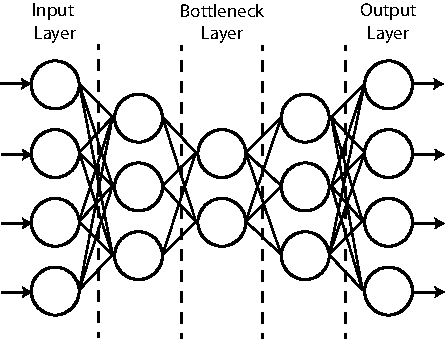
\includegraphics[width=\linewidth]{simple_autoencoder.pdf}
        \caption{Diagram representing a very basic autoencoder. It can be seen the the hidden layers introduces fewer and fewer nodes from the input layer. In doing so creates a bottle neck for the input data.}
        \label{fig:autoencoder}
    \end{figure}

\subsection{Optical Communication Link}
\subsection{Floating Point Arithmetic}